\documentclass{amsart}[12pt]
% \documentclass{usydthesis}[12pt]

\addtolength{\oddsidemargin}{-.75in}%
\addtolength{\evensidemargin}{-.75in}%
\addtolength{\textwidth}{1.5in}%
\addtolength{\textheight}{1.3in}%
\addtolength{\topmargin}{-.8in}%
\addtolength{\marginparpush}{-.75in}%
%\setlength\parindent{0pt}
%\setlength{\bibsep}{0pt plus 0.3ex}

\usepackage[authoryear]{natbib}
\usepackage[doublespacing]{setspace}
\usepackage{graphicx}
\usepackage{algorithm,algorithmic}
\usepackage{color}

\title{Collapsed Variational Approximation}
\author{Mark Greenaway}
% include.tex
\newcommand{\Bernoulli}[1]{\text{Bernoulli} \left( #1 \right)}
\newcommand{\mydigamma}[1]{\psi \left( #1 \right)}
%\newcommand{\diag}[1]{\text{diag}\left( #1 \right)}
\newcommand{\tr}[1]{\text{tr}\left( #1 \right)}
\newcommand{\Poisson}[1]{\text{Poisson} \left( #1 \right)}
\def \half {\frac{1}{2}}
\def \R {\mathbb{R}}
\def \vbeta {\vec{\beta}}
\def \vy {\vec{y}}
\def \vmu {\vec{\mu}}
\def \vmuqbeta {\vmu_{q(\vbeta)}}
\def \vmubeta {\vmu_{\vbeta}}
\def \Sigmaqbeta {\Sigma_{q(\vbeta)}}
\def \Sigmabeta {\Sigma_{\vbeta}}
\def \va {\vec{a}}
\def \vtheta {\vec{\theta}}
\def \mX {\vec{X}}

\def\ds{{\displaystyle}}

\def\diag{{\mbox{diag}}}


\usepackage{latexsym,amssymb,amsmath,amsfonts}
%\usepackage{tabularx}
\usepackage{theorem}
\usepackage{verbatim,array,multicol,palatino}
\usepackage{graphicx}
\usepackage{graphics}
\usepackage{fancyhdr}
\usepackage{algorithm,algorithmic}
\usepackage{url}
%\usepackage[all]{xy}



\def\approxdist{\stackrel{{\tiny \mbox{approx.}}}{\sim}}
\def\smhalf{\textstyle{\frac{1}{2}}}
\def\vxnew{\vx_{\mbox{{\tiny new}}}}
\def\bib{\vskip12pt\par\noindent\hangindent=1 true cm\hangafter=1}
\def\jump{\vskip3mm\noindent}
\def\etal{{\em et al.}}
\def\etahat{{\widehat\eta}}
\def\thick#1{\hbox{\rlap{$#1$}\kern0.25pt\rlap{$#1$}\kern0.25pt$#1$}}
\def\smbbeta{{\thick{\scriptstyle{\beta}}}}
\def\smbtheta{{\thick{\scriptstyle{\theta}}}}
\def\smbu{{\thick{\scriptstyle{\rm u}}}}
\def\smbzero{{\thick{\scriptstyle{0}}}}
\def\boxit#1{\begin{center}\fbox{#1}\end{center}}
\def\lboxit#1{\vbox{\hrule\hbox{\vrule\kern6pt
      \vbox{\kern6pt#1\kern6pt}\kern6pt\vrule}\hrule}}
\def\thickboxit#1{\vbox{{\hrule height 1mm}\hbox{{\vrule width 1mm}\kern6pt
          \vbox{\kern6pt#1\kern6pt}\kern6pt{\vrule width 1mm}}
               {\hrule height 1mm}}}


%\sloppy
%\usepackage{geometry}
%\geometry{verbose,a4paper,tmargin=20mm,bmargin=20mm,lmargin=40mm,rmargin=20mm}


%%%%%%%%%%%%%%%%%%%%%%%%%%%%%%%%%%%%%%%%%%%%%%%%%%%%%%%%%%%%%%%%%%%%%%%%%%%%%%%%
%
% Some convenience definitions
%
% \bf      -> vector
% \sf      -> matrix
% \mathcal -> sets or statistical
% \mathbb  -> fields or statistical
%
%%%%%%%%%%%%%%%%%%%%%%%%%%%%%%%%%%%%%%%%%%%%%%%%%%%%%%%%%%%%%%%%%%%%%%%%%%%%%%%%

% Sets or statistical values
\def\sI{{\mathcal I}}                            % Current Index set
\def\sJ{{\mathcal J}}                            % Select Index set
\def\sL{{\mathcal L}}                            % Likelihood
\def\sl{{\ell}}                                  % Log-likelihood
\def\sN{{\mathcal N}}                            
\def\sS{{\mathcal S}}                            
\def\sP{{\mathcal P}}                            
\def\sQ{{\mathcal Q}}                            
\def\sB{{\mathcal B}}                            
\def\sD{{\mathcal D}}                            
\def\sT{{\mathcal T}}
\def\sE{{\mathcal E}}                            
\def\sF{{\mathcal F}}                            
\def\sC{{\mathcal C}}                            
\def\sO{{\mathcal O}}                            
\def\sH{{\mathcal H}} 
\def\sR{{\mathcal R}}                            
\def\sJ{{\mathcal J}}                            
\def\sCP{{\mathcal CP}}                            
\def\sX{{\mathcal X}}                            
\def\sA{{\mathcal A}} 
\def\sZ{{\mathcal Z}}                            
\def\sM{{\mathcal M}}                            
\def\sK{{\mathcal K}}     
\def\sG{{\mathcal G}}                         
\def\sY{{\mathcal Y}}                         
\def\sU{{\mathcal U}}  


\def\sIG{{\mathcal IG}}                            


\def\cD{{\sf D}}
\def\cH{{\sf H}}
\def\cI{{\sf I}}

% Vectors
\def\vectorfontone{\bf}
\def\vectorfonttwo{\boldsymbol}
\def\va{{\vectorfontone a}}                      %
\def\vb{{\vectorfontone b}}                      %
\def\vc{{\vectorfontone c}}                      %
\def\vd{{\vectorfontone d}}                      %
\def\ve{{\vectorfontone e}}                      %
\def\vf{{\vectorfontone f}}                      %
\def\vg{{\vectorfontone g}}                      %
\def\vh{{\vectorfontone h}}                      %
\def\vi{{\vectorfontone i}}                      %
\def\vj{{\vectorfontone j}}                      %
\def\vk{{\vectorfontone k}}                      %
\def\vl{{\vectorfontone l}}                      %
\def\vm{{\vectorfontone m}}                      % number of basis functions
\def\vn{{\vectorfontone n}}                      % number of training samples
\def\vo{{\vectorfontone o}}                      %
\def\vp{{\vectorfontone p}}                      % number of unpenalized coefficients
\def\vq{{\vectorfontone q}}                      % number of penalized coefficients
\def\vr{{\vectorfontone r}}                      %
\def\vs{{\vectorfontone s}}                      %
\def\vt{{\vectorfontone t}}                      %
\def\vu{{\vectorfontone u}}                      % Penalized coefficients
\def\vv{{\vectorfontone v}}                      %
\def\vw{{\vectorfontone w}}                      %
\def\vx{{\vectorfontone x}}                      % Covariates/Predictors
\def\vy{{\vectorfontone y}}                      % Targets/Labels
\def\vz{{\vectorfontone z}}                      %

\def\vone{{\vectorfontone 1}}
\def\vzero{{\vectorfontone 0}}

\def\valpha{{\vectorfonttwo \alpha}}             %
\def\vbeta{{\vectorfonttwo \beta}}               % Unpenalized coefficients
\def\vgamma{{\vectorfonttwo \gamma}}             %
\def\vdelta{{\vectorfonttwo \delta}}             %
\def\vepsilon{{\vectorfonttwo \epsilon}}         %
\def\vvarepsilon{{\vectorfonttwo \varepsilon}}   % Vector of errors
\def\vzeta{{\vectorfonttwo \zeta}}               %
\def\veta{{\vectorfonttwo \eta}}                 % Vector of natural parameters
\def\vtheta{{\vectorfonttwo \theta}}             % Vector of combined coefficients
\def\vvartheta{{\vectorfonttwo \vartheta}}       %
\def\viota{{\vectorfonttwo \iota}}               %
\def\vkappa{{\vectorfonttwo \kappa}}             %
\def\vlambda{{\vectorfonttwo \lambda}}           % Vector of smoothing parameters
\def\vmu{{\vectorfonttwo \mu}}                   % Vector of means
\def\vnu{{\vectorfonttwo \nu}}                   %
\def\vxi{{\vectorfonttwo \xi}}                   %
\def\vpi{{\vectorfonttwo \pi}}                   %
\def\vvarpi{{\vectorfonttwo \varpi}}             %
\def\vrho{{\vectorfonttwo \rho}}                 %
\def\vvarrho{{\vectorfonttwo \varrho}}           %
\def\vsigma{{\vectorfonttwo \sigma}}             %
\def\vvarsigma{{\vectorfonttwo \varsigma}}       %
\def\vtau{{\vectorfonttwo \tau}}                 %
\def\vupsilon{{\vectorfonttwo \upsilon}}         %
\def\vphi{{\vectorfonttwo \phi}}                 %
\def\vvarphi{{\vectorfonttwo \varphi}}           %
\def\vchi{{\vectorfonttwo \chi}}                 %
\def\vpsi{{\vectorfonttwo \psi}}                 %
\def\vomega{{\vectorfonttwo \omega}}             %


% Matrices
%\def\matrixfontone{\sf}
%\def\matrixfonttwo{\sf}
\def\matrixfontone{\bf}
\def\matrixfonttwo{\boldsymbol}
\def\mA{{\matrixfontone A}}                      %
\def\mB{{\matrixfontone B}}                      %
\def\mC{{\matrixfontone C}}                      % Combined Design Matrix
\def\mD{{\matrixfontone D}}                      % Penalty Matrix for \vu_J
\def\mE{{\matrixfontone E}}                      %
\def\mF{{\matrixfontone F}}                      %
\def\mG{{\matrixfontone G}}                      % Penalty Matrix for \vu
\def\mH{{\matrixfontone H}}                      %
\def\mI{{\matrixfontone I}}                      % Identity Matrix
\def\mJ{{\matrixfontone J}}                      %
\def\mK{{\matrixfontone K}}                      %
\def\mL{{\matrixfontone L}}                      % Lower bound
\def\mM{{\matrixfontone M}}                      %
\def\mN{{\matrixfontone N}}                      %
\def\mO{{\matrixfontone O}}                      %
\def\mP{{\matrixfontone P}}                      %
\def\mQ{{\matrixfontone Q}}                      %
\def\mR{{\matrixfontone R}}                      %
\def\mS{{\matrixfontone S}}                      %
\def\mT{{\matrixfontone T}}                      %
\def\mU{{\matrixfontone U}}                      % Upper bound
\def\mV{{\matrixfontone V}}                      %
\def\mW{{\matrixfontone W}}                      % Variance Matrix i.e. diag(b'')
\def\mX{{\matrixfontone X}}                      % Unpenalized Design Matrix/Nullspace Matrix
\def\mY{{\matrixfontone Y}}                      %
\def\mZ{{\matrixfontone Z}}                      % Penalized Design Matrix/Kernel Space Matrix

\def\mGamma{{\matrixfonttwo \Gamma}}             %
\def\mDelta{{\matrixfonttwo \Delta}}             %
\def\mTheta{{\matrixfonttwo \Theta}}             %
\def\mLambda{{\matrixfonttwo \Lambda}}           % Penalty Matrix for \vnu
\def\mXi{{\matrixfonttwo \Xi}}                   %
\def\mPi{{\matrixfonttwo \Pi}}                   %
\def\mSigma{{\matrixfonttwo \Sigma}}             %
\def\mUpsilon{{\matrixfonttwo \Upsilon}}         %
\def\mPhi{{\matrixfonttwo \Phi}}                 %
\def\mOmega{{\matrixfonttwo \Omega}}             %
\def\mPsi{{\matrixfonttwo \Psi}}                 %

\def\mone{{\matrixfontone 1}}
\def\mzero{{\matrixfontone 0}}

% Fields or Statistical
\def\bE{{\mathbb E}}                             % Expectation
\def\bP{{\mathbb P}}                             % Probability
\def\bR{{\mathbb R}}                             % Reals
\def\bI{{\mathbb I}}                             % Reals
\def\bV{{\mathbb V}}                             % Reals

\def\vX{{\vectorfontone X}}                      % Targets/Labels
\def\vY{{\vectorfontone Y}}                      % Targets/Labels
\def\vZ{{\vectorfontone Z}}                      %

% Other
\def\etal{{\em et al.}}
\def\ds{\displaystyle}
\def\d{\partial}
\def\diag{\text{diag}}
%\def\span{\text{span}}
\def\blockdiag{\text{blockdiag}}
\def\tr{\text{tr}}
\def\RSS{\text{RSS}}
\def\df{\text{df}}
\def\GCV{\text{GCV}}
\def\AIC{\text{AIC}}
\def\MLC{\text{MLC}}
\def\mAIC{\text{mAIC}}
\def\cAIC{\text{cAIC}}
\def\rank{\text{rank}}
\def\MASE{\text{MASE}}
\def\SMSE{\text{SASE}}
\def\sign{\text{sign}}
\def\card{\text{card}}
\def\notexp{\text{notexp}}
\def\ASE{\text{ASE}}
\def\ML{\text{ML}}
\def\nullity{\text{nullity}}

\def\logexpit{\text{logexpit}}
\def\logit{\mbox{logit}}
\def\dg{\mbox{dg}}

\def\Bern{\mbox{Bernoulli}}
\def\sBernoulli{\mbox{Bernoulli}}
\def\sGamma{\mbox{Gamma}}
\def\sInvN{\mbox{Inv}\sN}
\def\sNegBin{\sN\sB}

\def\dGamma{\mbox{Gamma}}
\def\dInvGam{\mbox{Inv}\Gamma}

\def\Cov{\mbox{Cov}}
\def\Mgf{\mbox{Mgf}}

\def\mis{{mis}} 
\def\obs{{obs}}

\def\argmax{\operatornamewithlimits{\text{argmax}}}
\def\argmin{\operatornamewithlimits{\text{argmin}}}
\def\argsup{\operatornamewithlimits{\text{argsup}}}
\def\arginf{\operatornamewithlimits{\text{arginf}}}


\def\minimize{\operatornamewithlimits{\text{minimize}}}
\def\maximize{\operatornamewithlimits{\text{maximize}}}
\def\suchthat{\text{such that}}


\def\relstack#1#2{\mathop{#1}\limits_{#2}}
\def\sfrac#1#2{{\textstyle{\frac{#1}{#2}}}}


\def\comment#1{
\vspace{0.5cm}
\noindent \begin{tabular}{|p{14cm}|}  
\hline #1 \\ 
\hline 
\end{tabular}
\vspace{0.5cm}
}


\def\mytext#1{\begin{tabular}{p{13cm}}#1\end{tabular}}
\def\mytextB#1{\begin{tabular}{p{7.5cm}}#1\end{tabular}}
\def\mytextC#1{\begin{tabular}{p{12cm}}#1\end{tabular}}

\def\jump{\vskip3mm\noindent}

\def\KL{\text{KL}}
\def\N{\text{N}}
\def\Var{\text{Var}}

\def \E {\mathbb{E}}
\def \BigO {\text{O}}
\def \IG {\text{IG}}
\def \Beta {\text{Beta}}



\newcommand{\mgc}[1]{{\color{blue}#1}}
\newcommand{\joc}[1]{{\color{red}#1}}

\begin{document}
\setlength{\parindent}{0pt}
\maketitle

\section{Abstract}

Bayesian model selection is computationally expensive, and prone to getting stuck in local minima if the
posterior likelihood is multi-modal. This issue is particularly acute if the spike-and-slab prior,
particularly popular for Bayesian model selection, is used. We seek to address both problems by proposing a
population non-parametric Variational Bayes approximation algorithm - a population-based optimisation
strategy. Maintaining a population allows the posterior distribution to be explored more thoroughly, finding
multiple maxima. The variational approximation's lower bound includes an entropy term which ensures diversity
in the population by penalising similarity (the particles repel each other). This ensures the high probability
regions of the posterior distribution is thoroughly explored. This better reflects model selection
uncertainty.

\section{Introduction}

Bayesian model selection is a powerful set of techniques for model selection. These techniques are especially
useful in problems of high-dimension, such as bioinformatics problems where the model space is complex and
the optimal model is difficult for statisticians to manually specify.

In this article, we focus on the important case of model selection for normal linear models
\[
	p(\vy | \valpha, \vbeta) = \N_n(\vone^\top \alpha + \mX \vbeta, \mI_n)
\]
% Justify choice of prior

\cite{Mitchell1988} initially proposed the spike-and-slab prior distribution on regression co-efficients not
currently included in the model -- which places a mixture of a point mass 'spike' at $0$ and a diffuse uniform
distribution 'slab' elsewhere. The random error component is assigned a normal distribution with mean $0$ and
standard deviation $\sigma$. The approach was further developed by \cite{Madigan1994} to incorporate an
alternative Bayesian approach that takes full account of the true model uncertainty by averaging over a small
subset of models, and an efficient search algorithm for finding these models. \cite{George1997} investigated
computational methods for posterior evaluation and exploration in this setting, and using Gray Code sequencing
and Markov Chain Monte Carlo to explore the model space in moderate and large-sized problems respectively.
More recently, \cite{Ishwaran2005} developed a rescaled spike-and-slab model which improves effective variable
selection in terms of risk misclassification by using selective shrinkage. We further extend this approach, by
using the Cake variant of the spike-and-slab prior for model selection, as it avoids the Lindley and Bartlett
paradoxes. Citation.

Existing approaches to the problem of model selection focus upon finding a single best model quickly
(\cite{You2014}, \cite{Rockova2014}). Exploring the model space using only one model at a time will provide a
misleading view of the uncertainty in the posterior, as it is typically highly multimodal.

Many computational schemes for Bayesian model selection exist, using Monte Carlo Markov Chains techniques for 
computing the posterior distributions of $\vgamma$.
However, these schemes are both computationally intensive and can become trapped in local maxima of
the posterior distribution if the distribution is high-dimensional and multi-modal, as is the case with
popular choices of prior for Bayesian model selection problems, such as spike-and-slab priors. The difficulty
of becoming trapped in local maxima can be partially mitigated by using population-based MCMC schemes such
as Jasra et al. 2007, Bottolo and Richardson 2010, Hans et al 2007, Liang and Wong 2000. However, this
increases the computational cost of sampling from the posterior distributions still further, especially in
high-dimensional problems.

\cite{Rockova2016} introduced the notion of Particle EM. Rather than searching for a single optimal model,
Particle EM instead maintains a population of models (particles). This allows the algorithm to explore more of
the posterior model space, gaining a better estimate of the variation of the model space than an algorithm
involving only a single model. It also allows the particles to ``interact'', searching for the essential
posterior modes together. In Particle EM, this is done by incorporating an ``entropy term'' in the variational
lower bound, which ensures diversity amongst the models in the population, preventing all particles from
simply seeking the global posterior modes. The algorithm is determininistic.

We build upon this work by proposing a fixed-form parametric Variational Bayes approximation of $\vgamma$.
We adopt a prior structure incorporating the Cake prior for variable selection, which avoids the Lindley
and Bartlett's paradoxes.
Our fitting algorithm can be executed efficiently using rank-one updates and downdates.

Difficulty of implementation -- practical model selection
\cite{Chipman2014}

% Collapsed Variational Bayes
% Collapsed Variational Bayes approaches have proved useful in Bayesian nonparametric settings such as Latent
% Dirichlet Allocation \cite{Teh2007}
Our variational approximation is a fixed form parametric approximation which places a weight on each covariate
\[
	q(\vgamma) = \sum_{k=1}^K w_k \I(\vgamma_i)
\]

% Population-based MCMC approaches

Our main contributions are:

i) Our algorithm searches over the binary strings $\vgamma$ directly, as the estimates of $\vbeta$ are available 
in closed form once $\vgamma$ is known.

ii) We make use of a population--based optimisation scheme to search the model space. We take advantage of the
population of solutions by incorporating a penalty for lack of entropy.

iii) The entire trajectory of particles gives far more information about variable selection than a single
snapshot of the final best decision.

iv) Our model incorporates the Cake prior, which avoids Lindley's and Bartlett's paradoxes by selecting the
prior based on sample size.

This article is organised as follows. In Section 2, we detail the derivation of our approximation and fitting
algorithms. In Section 3, we discuss computational issues with implementing our algorithm efficiently. In
Section 4, we present the results of our numerical experiments. In Section 5, we present our conclusions and
discuss our results.

\section{Method}

Base on John's CVB for Mark document.

The main body of the algorithm is a two--stage process. In the first stage, we iterate through the population of
bitstrings, using a greedy search strategy to attempt to alter each bit in the model bitstring to increase the log likelihood. If the log likelihood for the new bitstring is no higher than the previous bitstring, then the
alteration is rejected and the next alteration tried. The alterations are also rejected if the new bitstring
already exists within the population, ensuring that the constraint that all models in the population are
unique is maintained.

In the second stage, we re--calculate the weights for each individual in the population, based on the
likelihood of that model relative to the data $p(\vy; \vbeta_\vgamma)$ and the use this to re--calculate the
probability--based weights $w_i$ for each bitstring in the population. This is then used to re--calculate the
lower bound
\[
	\log \underline{p}(\vy; \vw, \Gamma) = \sum_{k=1}^K \vw_k \log p(\vy; \vbeta_{\vgamma_k}) - \vw_k \log \vw_k
\]

which is the sum of the weighted log-likelihood of the population and the entropy of the probability weights.
These two stages repeat until the lower bound converges.

\section{Results}

If the covariates in a model selection problem are highly collinear then the posterior distribution will be
highly multi-modal when a spike-and-slab prior structure is used. This can make seeking the optimal model very
challenging, due to the many local optima. In this section, we present a series of numerical experiments which
demonstrate the capability of our algorithm to successfully find the models with high posterior probability in
such situations.

We first present an example where $n > p$ and $p$ is relatively small ($p = 12$), to allow for the full 
enumeration of the model space. Later, we show an example for the important $p > n$ case, and compare our results 
against the xxx algorithm.

The results were generated by repeatedly simulating the data set $1,000$ times and fitting the CVA model.
The median posterior model probability was calculated by taking the median across all of the runs of the
total posterior probability of all of the models discovered by the CVA algorithm during that run. The global
percentage was the proportion of the runs where the CVA algorithm successfully found the global mode.

\subsection{$n > p$}

Our first numerical experiment is designed to show that our algorithm successfully finds the posterior models
of high probability, overcoming the difficulties of optimising over the multi-modal spike-and-slab posterior.
We consider a random sample of $n = 50$ observations on $p = 12$ predictors. $\mX_i \sim \N_p(\vzero, \mSigma)$
for $i = 1, \ldots, n$ where
$\mSigma = \text{bdiag}(\mSigma_1, \mSigma_1, \mSigma_1, \mSigma_1)$ with
$\mSigma_1 = (\sigma_{ij})_{i, j = 1}^{3, 3}$ where $\sigma_{ij} = 0.9$ for $i \ne j$ and $\sigma_{ii} = 1$.
The true model is $\vbeta_0 = (1.3, 0, 0, 1.3, 0, 0, 1.3, 0, 0, 1.3, 0, 0)^\top$.
The responses are then generated from $\vy = \mX \vbeta_0 + \vepsilon$, where
$\vepsilon \sim \N_n(\vzero, \mI_n)$.

\subsection{CVA}

\subsubsection{Experiment 1}
Figure \ref{fig:posterior_model_probabilities} shows all $4,096$ posterior model probabilities ordered by the
model's bit strings. We can clearly see a few peaks in the full posterior distribution. Our experiment aims to
show that most of these posterior peaks are successfully identified by our algorithm.

We begin by using the setting $\lambda = 1$, allowing particle repulsion between each of the models within the
population. Our population of bit strings $\mGamma^{(0)} = [\vgamma_1^{(0)}, \ldots, \vgamma_K^{(0)}]$ with
$K = 20$ particles was randomly initialised from a sequencial of independent Bernoulli trials with probability
of success $1/2$.

\begin{figure}
	\caption{Posterior model probabilities when $p = 12$. Red circles denote models visited by the CVA
						algorithm, while black circles are models that were not visited.}
	\label{fig:posterior_model_probabilities}
	\includegraphics[scale=0.75]{code/correlation/cva_low_dimensional.pdf}
\end{figure}

\begin{figure}
	\caption{Posterior model probabilities when $p = 21$. Red circles denote models visited by the CVA
						algorithm, while black circles are models that were not visited.}
	\label{fig:posterior_model_probabilities2}
	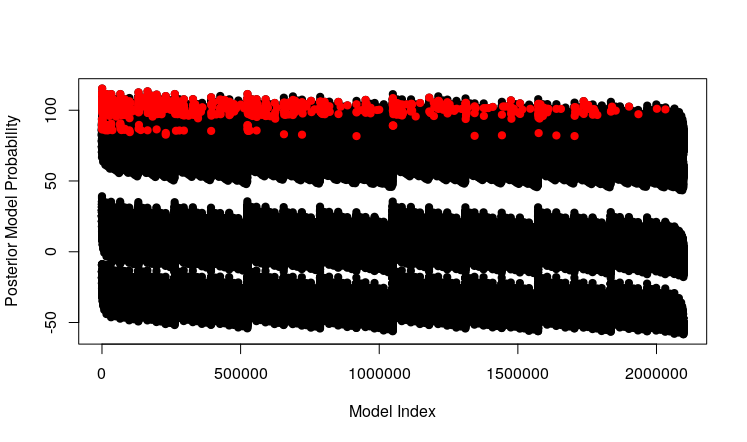
\includegraphics[scale=0.75]{code/correlation/cva_more_dimensions.pdf}
\end{figure}

\begin{figure}
	\caption{Comparison of covariate inclusion probabilities for CVA versus EMVS}
	\label{fig:covariate_inclusion_probabilities}
	\includegraphics[scale=0.75]{code/correlation/covariate_inclusion_probabilities.pdf}
\end{figure}

\subsection{$p > n$}

\begin{table}
	\caption{}
	\label{tab:result2}
	\begin{tabular}{l|llll|llll|llll|llll}
	\hline
	 					& \multicolumn{4}{c}{K=20} 	& \multicolumn{4}{c}{K=50} & \multicolumn{4}{c}{K=100} \\
	$\lambda$ & 0 & 1 & 2 & 3 & 0 & 1 & 2 & 3 & 0 & 1 & 2 & 3 & 0 & 1 & 2 & 3 \\
	\hline
	\# Modes & \\
	\% Posterior & 83.1 & 84.7 & 83.7 & 82.3 & 84.7 & 83.2 & 85.4 & 84.8 & 81.9 & 82.9 & 83.9 & 84.6 & 83.9 & 81.5 & 82.0 & 85.2 \\
	\% Global Mode & 91 & 90 & 87 & 82 & 86 & 85 & 80 & 90 & 90 & 90 & 86 & 91 & 88 & 91 & 76 & 88 \\
	\hline
	\end{tabular}

\end{table}

% Show posterior probabilities on the log scale
In the plots of the log posterior probabilities of the models, the particles can be seen clustering at the
highest probability models first, then spreading through the medium and low probability models. From these
plots we can see that once $K$ is high enough, there is a good variety of high, medium and low posterior
probability models in the population of particles.

\section{Implementation techniques}
Our model updates are made efficient by using rank-one updates to update the inverse of $(\mX^\top \mX)^{-1}$.

To ensure uniqueness of the $K$ models in the population, before a new candidate model with a covariate added
or removed is considered, the population of existing models is checked to see if it already exists in the
population. If so, the addition or removal of the covariate is skipped and the next candidate model considered.
In our implementation, this check is made computationally efficient by maintaining a hash table of the models,
allowing the check as to whether the model is already in the population to be performed in $\BigO(1)$ time.

\bibliographystyle{elsarticle-harv}
\bibliography{references_mendeley}

\end{document}
